\documentclass{article}
\pagestyle{empty}
%\usepackage{geometry,fontspec,tikz}
\usepackage[svgnames]{xcolor}
\usepackage{tikz}
\newcommand{\h}[1]{\textcolor{FireBrick}{#1}}
\usepackage{pdfpages}

\usepackage{geometry}
\geometry{a6paper,landscape,hmargin={1cm,1cm},vmargin={1cm,1cm}}
%\usepackage[letterpaper, top=0in, bottom=0in, left=0in, right=0in]{geometry}


%\setmainfont[Ligatures=TeX]{Adobe Garamond Pro}
\usetikzlibrary{fadings}
\tikzfading[name=fade right,
left color=transparent!0,
right color=transparent!100]
\setlength\parindent{0pt}

\usepackage{calc}
\usepackage{fontawesome}
\usepackage[colorlinks=true, linkcolor=Maroon, urlcolor=Maroon]{hyperref}

\newcommand*{\pin}{%
  
\includegraphics[height=\heightof{M}]{pin}%
}

\begin{document}

\includepdf[width=\paperwidth, height=\paperheight]{/home/sm/Documents/Weddding-Invitation/test4.pdf}

\begin{tikzpicture}[overlay,remember picture]
  \node[anchor=east,inner sep=0pt] (pic) at (current page.east)
    {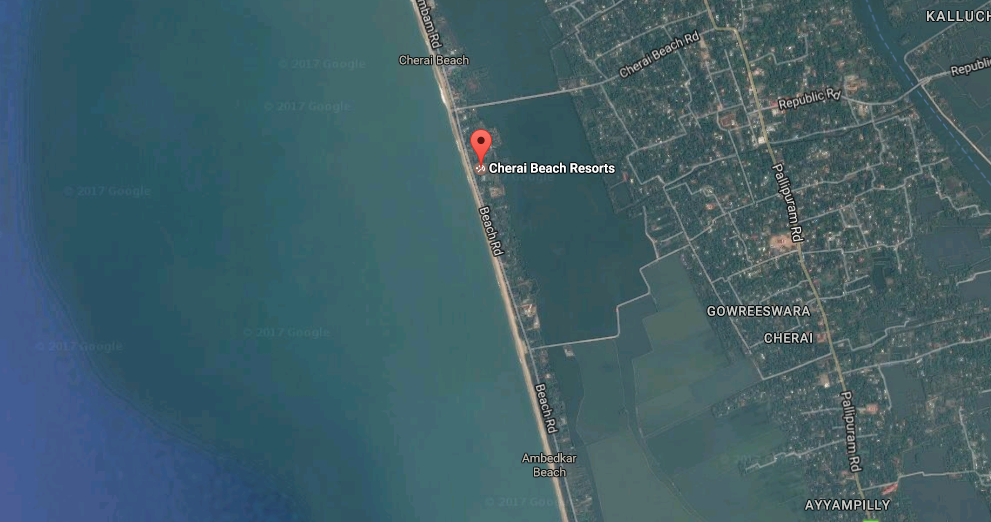
\includegraphics[width=1.001\paperwidth,height=\pdfpageheight]{map_satellite}};
  \fill[white,path fading=fade right] (pic.north west) rectangle (pic.south east);
  \coordinate (pin) at (6.15,-1.8);
  \filldraw[draw=Maroon,fill=Maroon!70] (pin) -- ++(70:.5) arc (-20:200:.18) -- cycle;
  \path (pin) -- ++(0,.5) node[draw,fill,Maroon,circle,inner sep=1pt] {};
\end{tikzpicture}%
\obeylines%
%{\addfontfeatures{Scale=3,LetterSpace=10} INVITATION}
{\huge{\textsc{\h{V}enue}}}
\bigbreak
{\small \emph\textit{%
\textbf{\textsc{\h{C}herai \h{B}each \h{R}esorts}}
Vypin Island
Kochi, Kerala
Pin - 683514 
}}

\vfill

{\small \emph \textit{%
  \scshape \textbf{\h{O}n}: \textbf{\h{J}une \h{1}0}\/\rlap{,}\textsuperscript{th} \textbf{\h{2}017}
  \textbf{\h{A}t: }\textbf{11}\kern.5pt:\kern.5pt\textbf{30 am}
}}


\vfill

\medbreak
%{\addfontfeatures{Scale=1.4,LetterSpace=5}\scshape where?}
{\scshape \textbf{\h{D}irections}}
\begin{itemize}
	\item []Click any of the links below \\to get directions on Google Maps
\end{itemize}

\begin{itemize}
	\item[] {\normalsize \pin} \underline{\href{https://www.google.co.in/maps/dir/Mount+Carmel+Church,+Pottakuzhi+-+Mamangalam+Rd,+Mamangalam,+Elamakkara,+Ernakulam,+Kerala+682025/Cherai+Beach+Resorts,+Cherai,+Vypin,+Kerala/@10.0633394,76.1809834,12z/data=!3m1!4b1!4m13!4m12!1m5!1m1!1s0x3b080d0fa96af125:0x696a9989e82b6c02!2m2!1d76.3032795!2d10.0093666!1m5!1m1!1s0x3b0810a300000001:0xebdd3e12cda825ee!2m2!1d76.1986595!2d10.1363985}{From Ernakulam}}

	\item[] {\normalsize \pin} \underline{\href{https://www.google.co.in/maps/dir/Aluva+Railway+Station,+Periyar+Nagar,+Aluva,+Kerala/Cherai+Beach+Resorts,+Cherai,+Vypin,+Kerala/@10.126786,76.2902413,13.25z/data=!4m13!4m12!1m5!1m1!1s0x3b080f29eb7eb615:0xb454e4d93b04846c!2m2!1d76.3567139!2d10.1086654!1m5!1m1!1s0x3b086d34d768e025:0x4fa5702ae301f77f!2m2!1d76.1805941!2d10.1363345}{From Aluva}}
	\item[] {\normalsize \pin} \underline{\href{https://www.google.co.in/maps/dir/Kodungallur+Bhagavathy+Temple,+Kodungallur,+Kerala/Cherai+Beach+Resorts,+Cherai,+Vypin,+Kerala/@10.1821016,76.1630008,13z/data=!3m1!4b1!4m13!4m12!1m5!1m1!1s0x3b081bf47f4c042f:0x7e6f994f0db02349!2m2!1d76.1984602!2d10.2268941!1m5!1m1!1s0x3b086d34d768e025:0x4fa5702ae301f77f!2m2!1d76.1805941!2d10.1363345}{From Kodungallur}}
\end{itemize}
\end{document}